\documentclass[12pt]{article}
\usepackage{natbib,amsmath,amsfonts,fullpage,hyphenat,booktabs,graphicx,setspace}
\usepackage[colorlinks,linkcolor=blue,citecolor=blue,urlcolor=blue]{hyperref}
\setcitestyle{square,super,comma}

\title{Reading report\\Randomized kinodynamic motion planning with moving obstacles\cite{hsu2002randomized}}
\author{Dharmin Bakaraniya}
\begin{document}
\maketitle{}

\begin{abstract}
This paper presents a novel randomized motion planner for robots
that must achieve a specified goal under kinematic and/or dynamic
motion constraints while avoiding collision with moving obstacles
with known trajectories. The planner encodes the motion constraints
on the robot with a control system and samples the robot’s state×time
space by picking control inputs at random and integrating its equations of motion. The result is a probabilistic roadmap of sampled
state×time points, called milestones, connected by short admissible trajectories. The planner does not precompute the roadmap;
instead, for each planning query, it generates a new roadmap to
connect an initial and a goal state×time point. The paper presents a
detailed analysis of the planner’s convergence rate. It shows that, if
the state×time space satisfies a geometric property called expansiveness, then a slightly idealized version of our implemented planner
is guaranteed to find a trajectory when one exists, with probability
quickly converging to 1, as the number of milestones increases. Our
planner was tested extensively not only in simulated environments,
but also on a real robot. In the latter case, a vision module estimates
obstacle motions just before planning starts. The planner is then
allocated a small, fixed amount of time to compute a trajectory. If
a change in the expected motion of the obstacles is detected while
the robot executes the planned trajectory, the planner recomputes
a trajectory on the fly. Experiments on the real robot led to several
extensions of the planner in order to deal with time delays and uncertainties that are inherent to an integrated robotic system interacting
with the physical world.
\end{abstract}

\section{Summary}
\begin{itemize}
    \item The author states that their work extends \textit{probabilistic roadmap} (PRM) framework\cite{kavraki1996}.
    \item ``A PRM planner samples the robot’s configuration space at
        random and retains the collision-free samples as milestones.
        It then tries to connect pairs of milestones with paths of pre-defined shape (typically straight-line segments in configura-
        tion space) and retains the collision-free connections as local
        paths. The result is an undirected graph, called a probabilistic roadmap, whose nodes are the milestones and the edges
        are the local paths''\cite{hsu2002randomized}
    \item The authors state that they hace extended the PRM framework with kinodynamic constraints on controls and by providing mathematical proofs and bounds along with experimental results.
    \item Kinodynamic constraints is a set of differential equation which describe all the possible motion that the robot can make given its current configuration and velocity.
    \item The authors consider the robots whose motion constraints can be expressed as $$\dot s = f(s, u)$$ where $s \epsilon S$ and $u \epsilon \Omega$, $S$ is \textit{state space} and $\Omega$ is \textit{control space}.
    \item This motion constraints cover most of the vehicles (holonomic and non holonomic) including cars, differential drive robots and even more complex vehicles like two robots connected with link.
    \item This algorithm provides a basic use of this approach
        \begin{figure}[ht!]
            \centering
            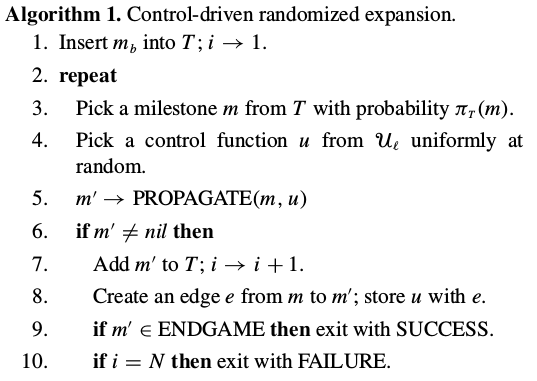
\includegraphics[width=0.6\linewidth]{algo.png}
            \caption{Basic algorithm for kinodynamic motion planning\label{fig:basicAlgo}}
        \end{figure}
    \item PROPOGATE integrates the equation from \textit{m} with control \textit{u}. If the computed trajectory is admissible, then it return a \textit{milestone m'}, otherwise it returns \textit{nil}.
    \item ENDGAME is a region around goal. As it is very difficult for a robot to reach exact goal position, generally the robot is considered to have reached the goal when it is in a surrounding area of the actual goal position.
    \item N is the upper bound on the number of milestones that the algorithm is allowed to expand. If the alogrithm is not able to find a trajectory from current position to goal area within N milestones, then the algorithm returns \textit{fail} result.
    \item The probability ($\pi_T$) for choosing a milestone at line 3 is inversely proposional to the amount of milestones present in surrounding area. This approach for choosing a milestone was proved by the author to work not only faster than the existing technique of rejection sampling but also better for this application. The reason why this was better for this application is because an actual uniform distribution is not required for this algorithm.
    \item The authors prove that the probability of finding a trajectory to goal area converges to 1 exponentially as the number of milestones increases. $$r \ge \frac{\ln(2/g)}{\alpha \beta} \cdot \ln \frac{2\ln(2/g)}{\beta \gamma} + \frac{2}{g}\ln\frac{2}{\gamma}$$
        where $r$ is the number of milestones, $g$ is the area around goal, $\alpha$ and $\beta$ are constants that determine expansive nature of algorithm and $\gamma$ is a constant in range (0,1].
    \item The author confess that eventhough they found out the nature in which the algorithm behaves based on the number of milestones, they still are not able to choose the correct value of $\alpha$ and $\beta$.
    \item The authors have performed experiments on 2 different models of robot
        \begin{itemize}
            \item Two cart non-holonomic robot
            \item Air cushioned robot (holonomic).
        \end{itemize}
    \item For two cart robot, they ran the simulation on 3 different scenarios, maze, narrow passage and home environment. For a single iteration, the algorithm runs for less than a second most of the time. Here the environment is kept static.
    \item For air cushioned robot, 2 types of tests were performed
        \begin{itemize}
            \item \textbf{Simulation}: The robot was faced with 3 different scenarios. In all of them the algorithm ran around 0.2 seconds for single interation. There were 5 moving obstacles in each of these scenarios.
            \item \textbf{Real robot}: For detecting the position and velocity of obstacles, LEDs were placed on obstacles, which provided information at 60Hz ot the robot. The planner run offline. Due to data overheads, the author decided to give the planner, an extra 0.4 seconds. The robot was able to successfully come up with trajectories for all scenarios.
        \end{itemize}
    \item For experimenting with a real robot, the authors developed some additional techniques that helped with the performance of the planner.
        \begin{itemize}
            \item \textit{Trajectory tracking}: Because of errors in sensor, the planner grows the obstacle boundaries.
            \item \textit{Trajectory optimization}: If the planner has more time after searching a valid trajectory, it searches additional trajectories and returns the best one. This reduced the cost of trajectories by 14\%.
            \item \textit{Safe mode planning}: If a valid trajectory was not found in the alloted time, then the robot will not just sit there and wait for collision. It calculates an escape route along with route towards goal. This increases the planning time by 2\% but ensures safety.
            \item \textit{On-the-fly replanning}: If the direction or velocity of the obstacle changes while the robot is executing the plan, the planner recomputes another trajectory. This is possible because the planner is given information 0.4 seconds in future by the perception module. This additional time is more than enough for the robot to replan.
        \end{itemize}
\end{itemize}

\section{Scientific contributions}
\begin{itemize}
    \item A significant extension of existing PRM approach.
    \item Mathematical proof showing that the probability of finding trajectory to goal converges to 1 exponentially with increasing milestones.
    \item Experimental proof of PRM approach. The approach was demonstrated not only on circular holonomic robot but also on non-holonomic robot (a collection of 2 holonomic robot connected with a link).
    \item Some additional heuristic and techniques to perform the experiment on real robot.
\end{itemize}

\section{Scientific deficits}
\begin{itemize}
    \item The computation increases very much even for medium number of moving obstacles.
    \item The approach does not guarantee to find the path to the target even if it exists because of timeout.
\end{itemize}

\begin{thebibliography}{1}
    \bibitem{hsu2002randomized} Hsu, D.; Kindel, R.; Latombe, J.-C. \& Rock, S. ``Randomized kinodynamic motion planning with moving obstacles'', \textit{The International Journal of Robotics Research}, 2002.
    \bibitem{kavraki1996} Kavraki, L., Švestka, P., Latombe, J. C., and Overmars, M. H. ``Probabilistic roadmaps for path planning in high-dimensional configuration space''. \textit{IEEE Transactions on Robotics and Automation}, 1996.
\end{thebibliography}

\end{document}
